\section{Experimental evaluation}
\label{Sec:experimental-eval}

Here we report the results of the tests executed to compare the performances between the sequential and parallel versions of A*.
\\
All the tests were performed on a Linux environment.

\subsection{Time performance}

To test the parallel A* algorithm we changed the number of threads and the function used to compute the recipient (\ref{compute_reci}), while using the same input data (same map, same starting node and destination node),
then we compared the results with the ones from sequential A*. 

\subsubsection{Grid Milan}
The graph generated from the grid of Milan (1024x1024) has around 800k nodes and has randomly generated weights to increase the difficulty to find the path with the best cost.
\\
The Figure \ref{Milan-grid} represents a drawing of the path found by the algorithms with the data that we used for testing.

\begin{center} 
    \begin{minipage}[b]{0.3\textwidth}
        \centering
        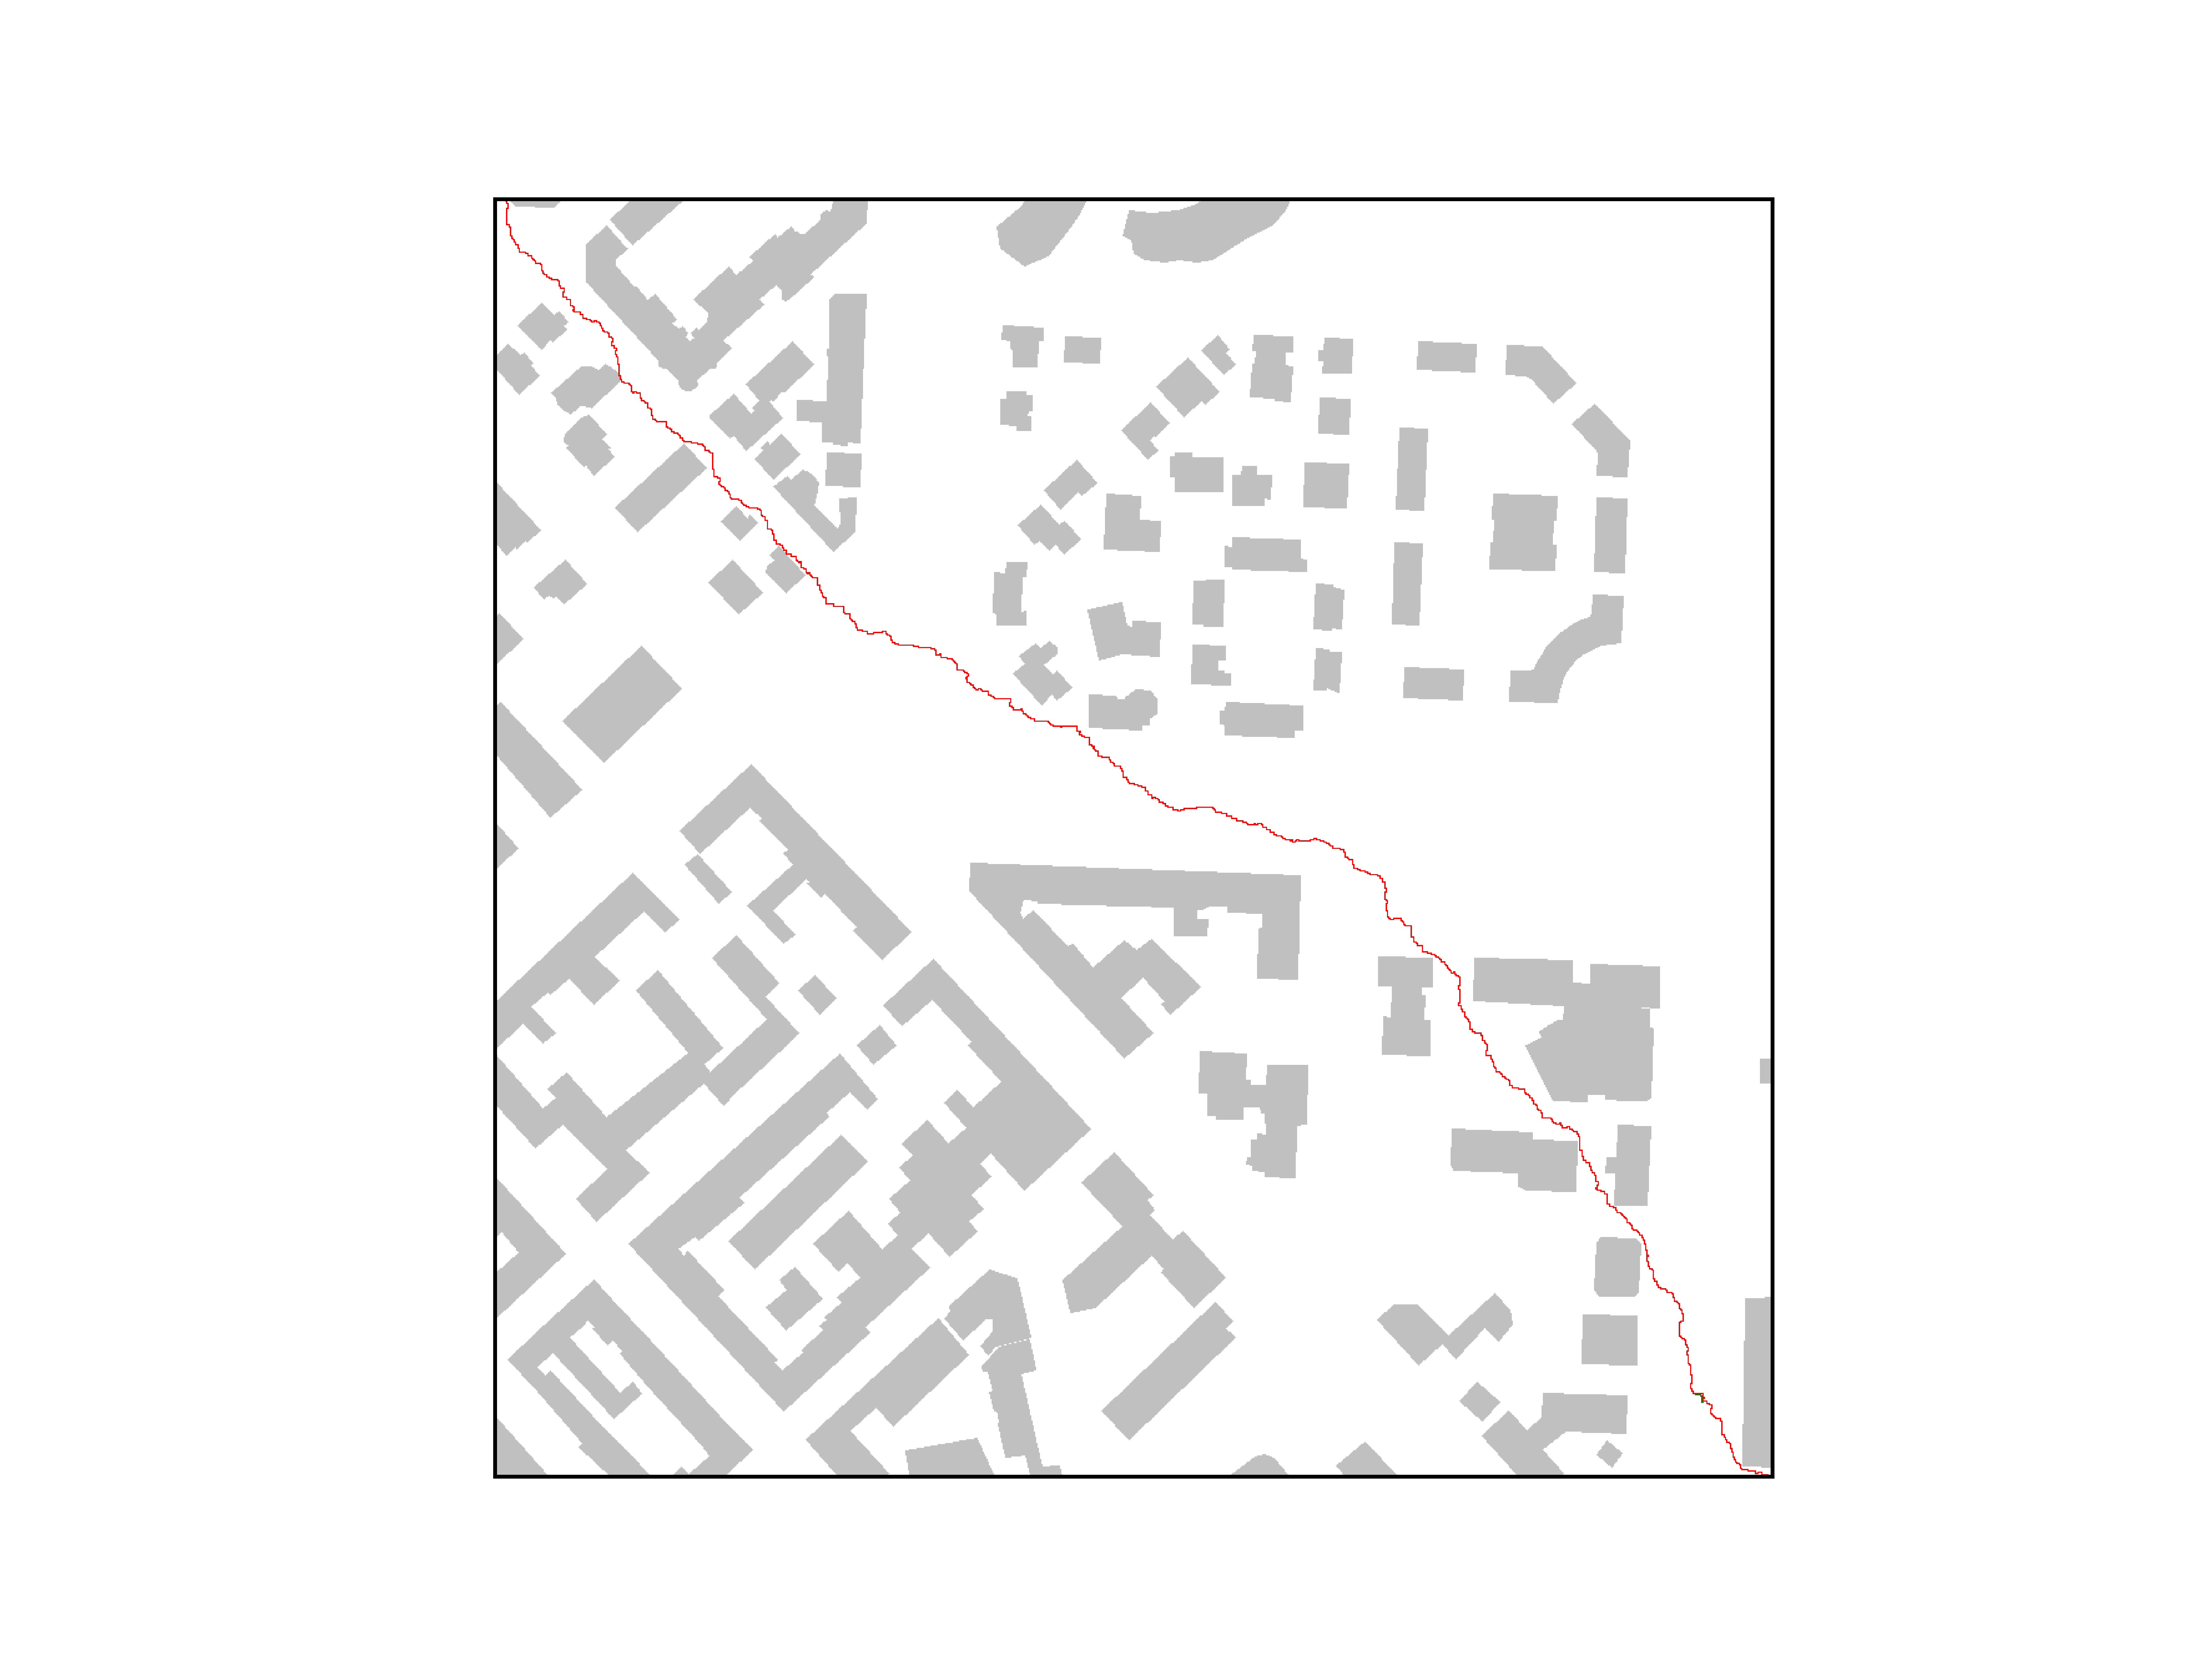
\includegraphics[scale=0.5]{gridMilan.png}
        \captionof{figure}{Milan map with path found}
        \label{Milan-grid}
    \end{minipage}%
    \hspace{0.5cm}
    \begin{minipage}[b]{0.6\textwidth}
        \centering
        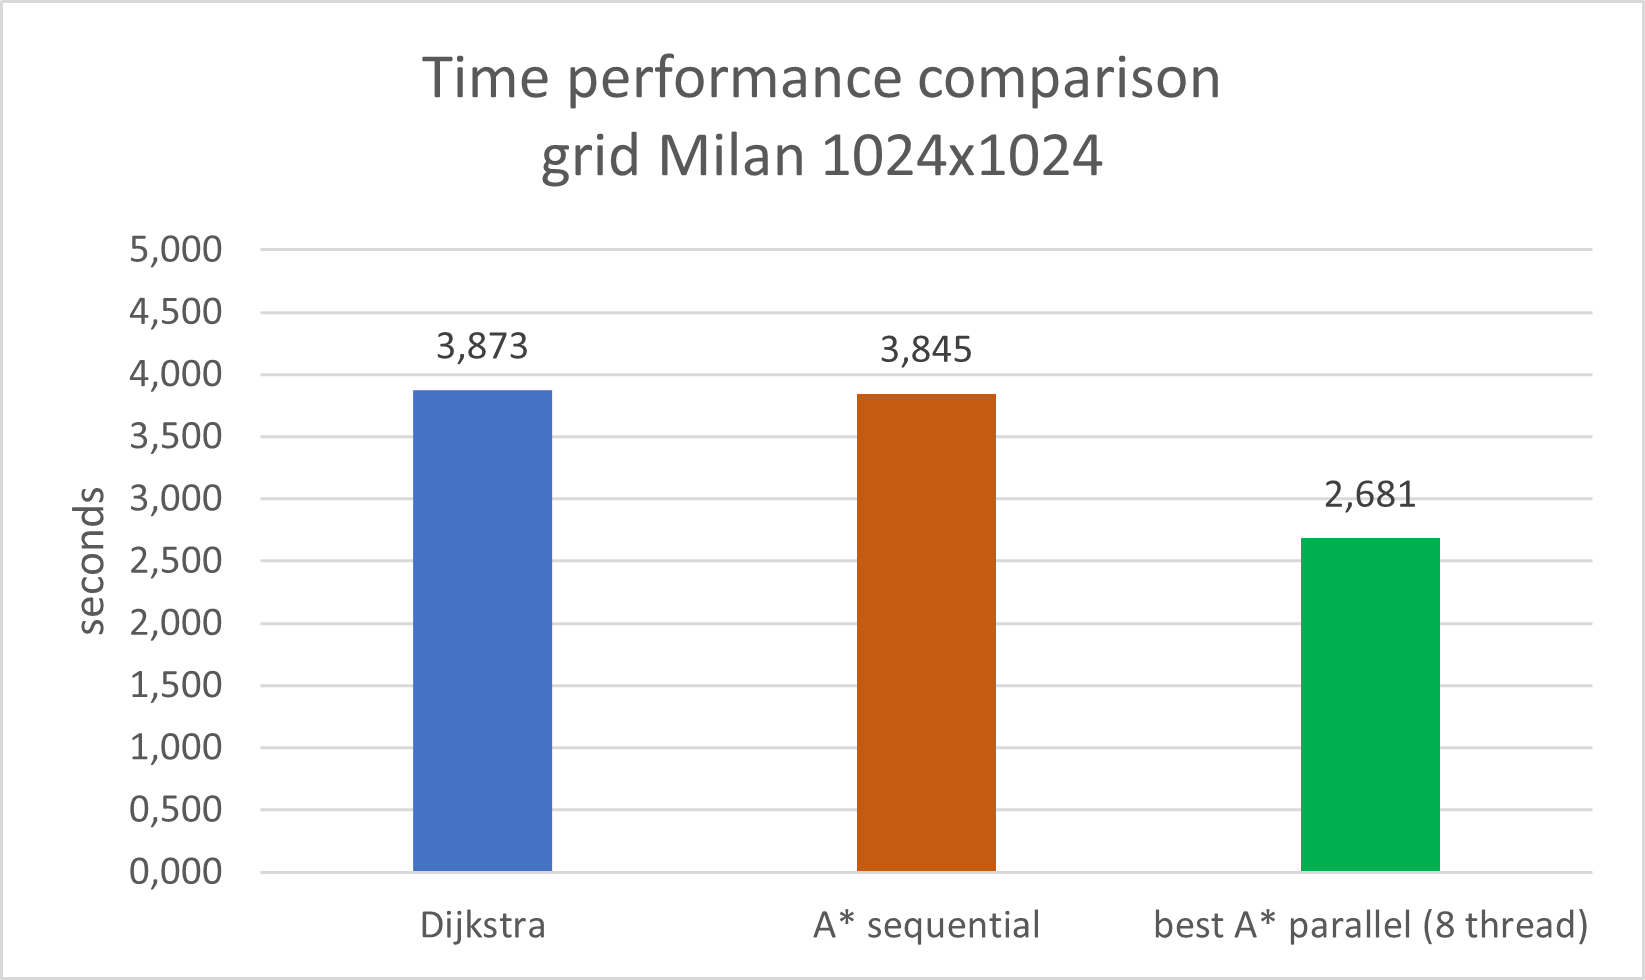
\includegraphics[scale=0.7]{milanComparison.png}
        \captionof{figure}{Performance comparison between different algorithms on grid Milan}
        \label{Milan-comp}
    \end{minipage} 
\end{center}
Looking at Figure \ref{Milan-comp}, and taking into account that we chose the most efficient number of threads for parallel A*,
we can notice a better performance compared to the sequential A* and the Dijkstra algorithms.
\\ 
In order to find the best result, we tried parallel A* changing the number of threads and the compute recipient function:
Figure \ref{Milan-par-comp} shows all the experimental results of the tests.
\\
Comparing the two compute recipient functions (simple module and multiplicative hash)
on this relatively small graph, it can be observed that when running with limited number of threads the performances are similar.
\\
With the increase of the level of parallelism the performances are no longer comparable, and the algorithm with multiplicative hash function is faster.

\begin{figure}
    \centering
    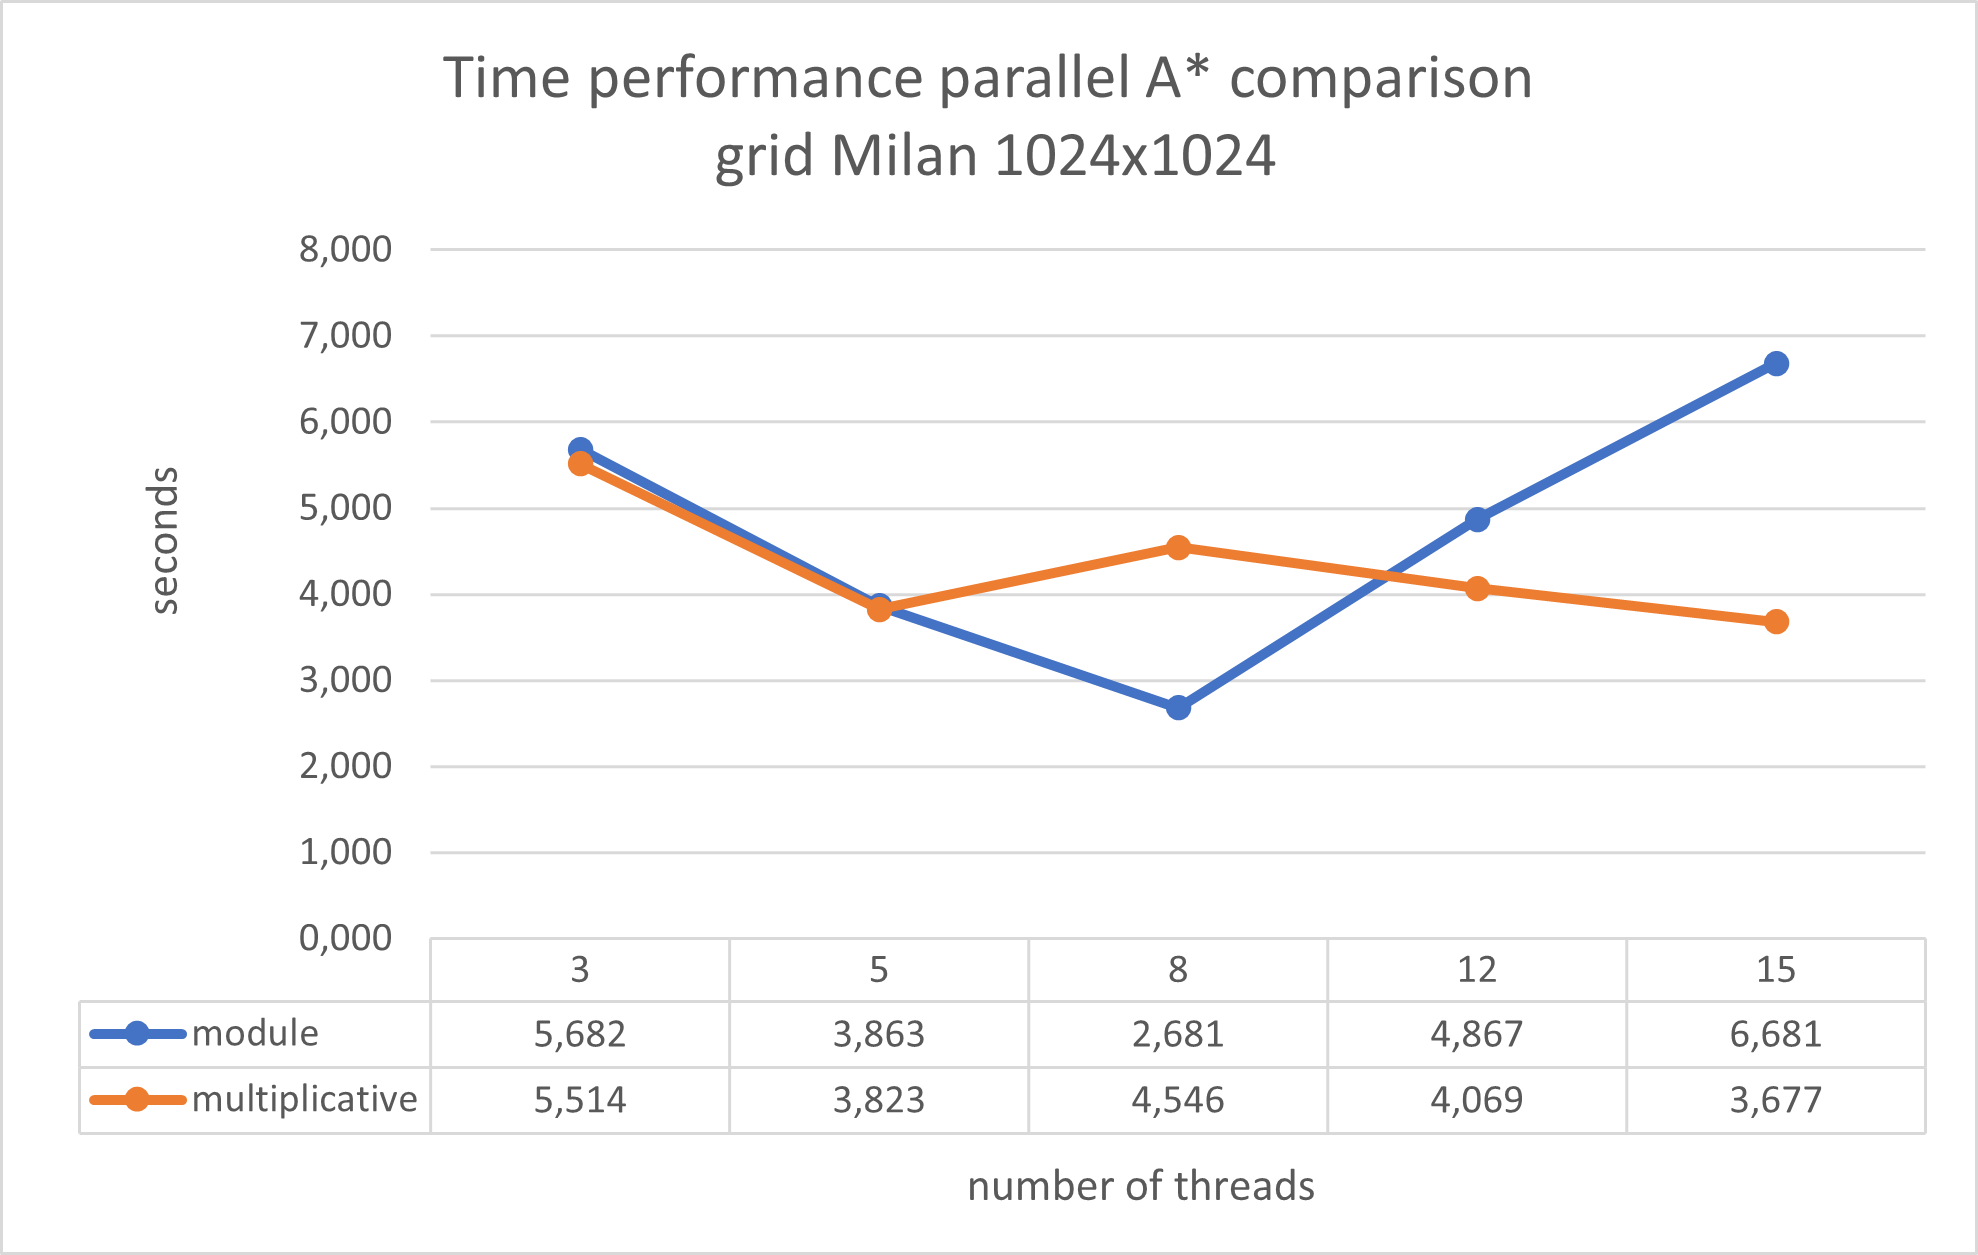
\includegraphics[scale=0.7]{milanParComparison.png}
    \caption{Performance comparison with different number of threads and compute recipient function}
    \label{Milan-par-comp}
\end{figure}

\newpage

\subsubsection{Large Map}

To better test our algorithms we used larger graphs, always with random weights, with about 4 Millions nodes.

\begin{center} 
    \begin{minipage}[b]{0.45\textwidth}
        \centering
        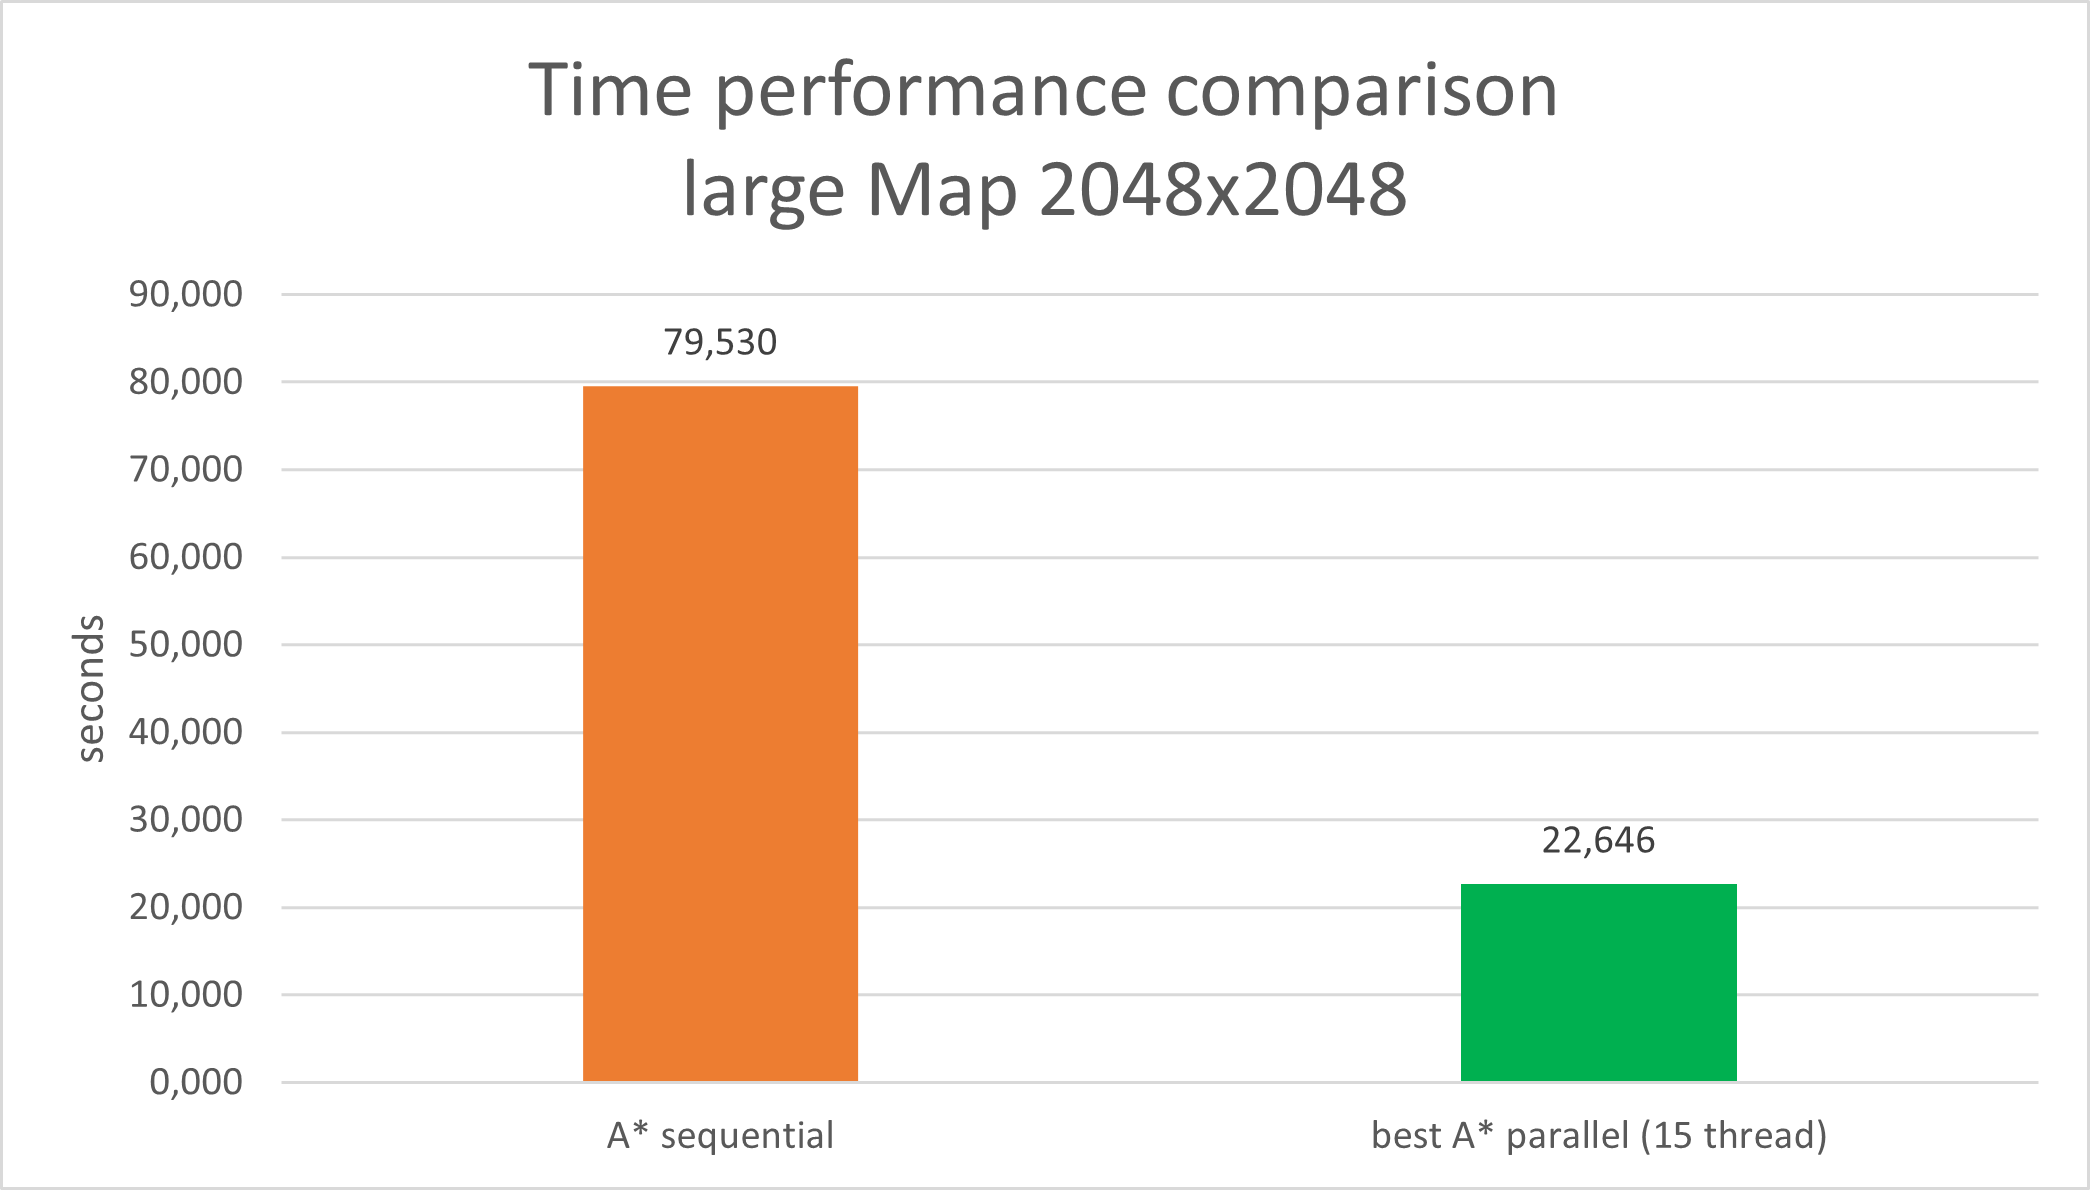
\includegraphics[scale=0.45]{mapComparison.png}
        \captionof{figure}{Performance comparison between different algorithms on large map}
        \label{Map-comp}
    \end{minipage} 
    \hspace{0.5cm}
    \begin{minipage}[b]{0.45\textwidth}
        \centering
        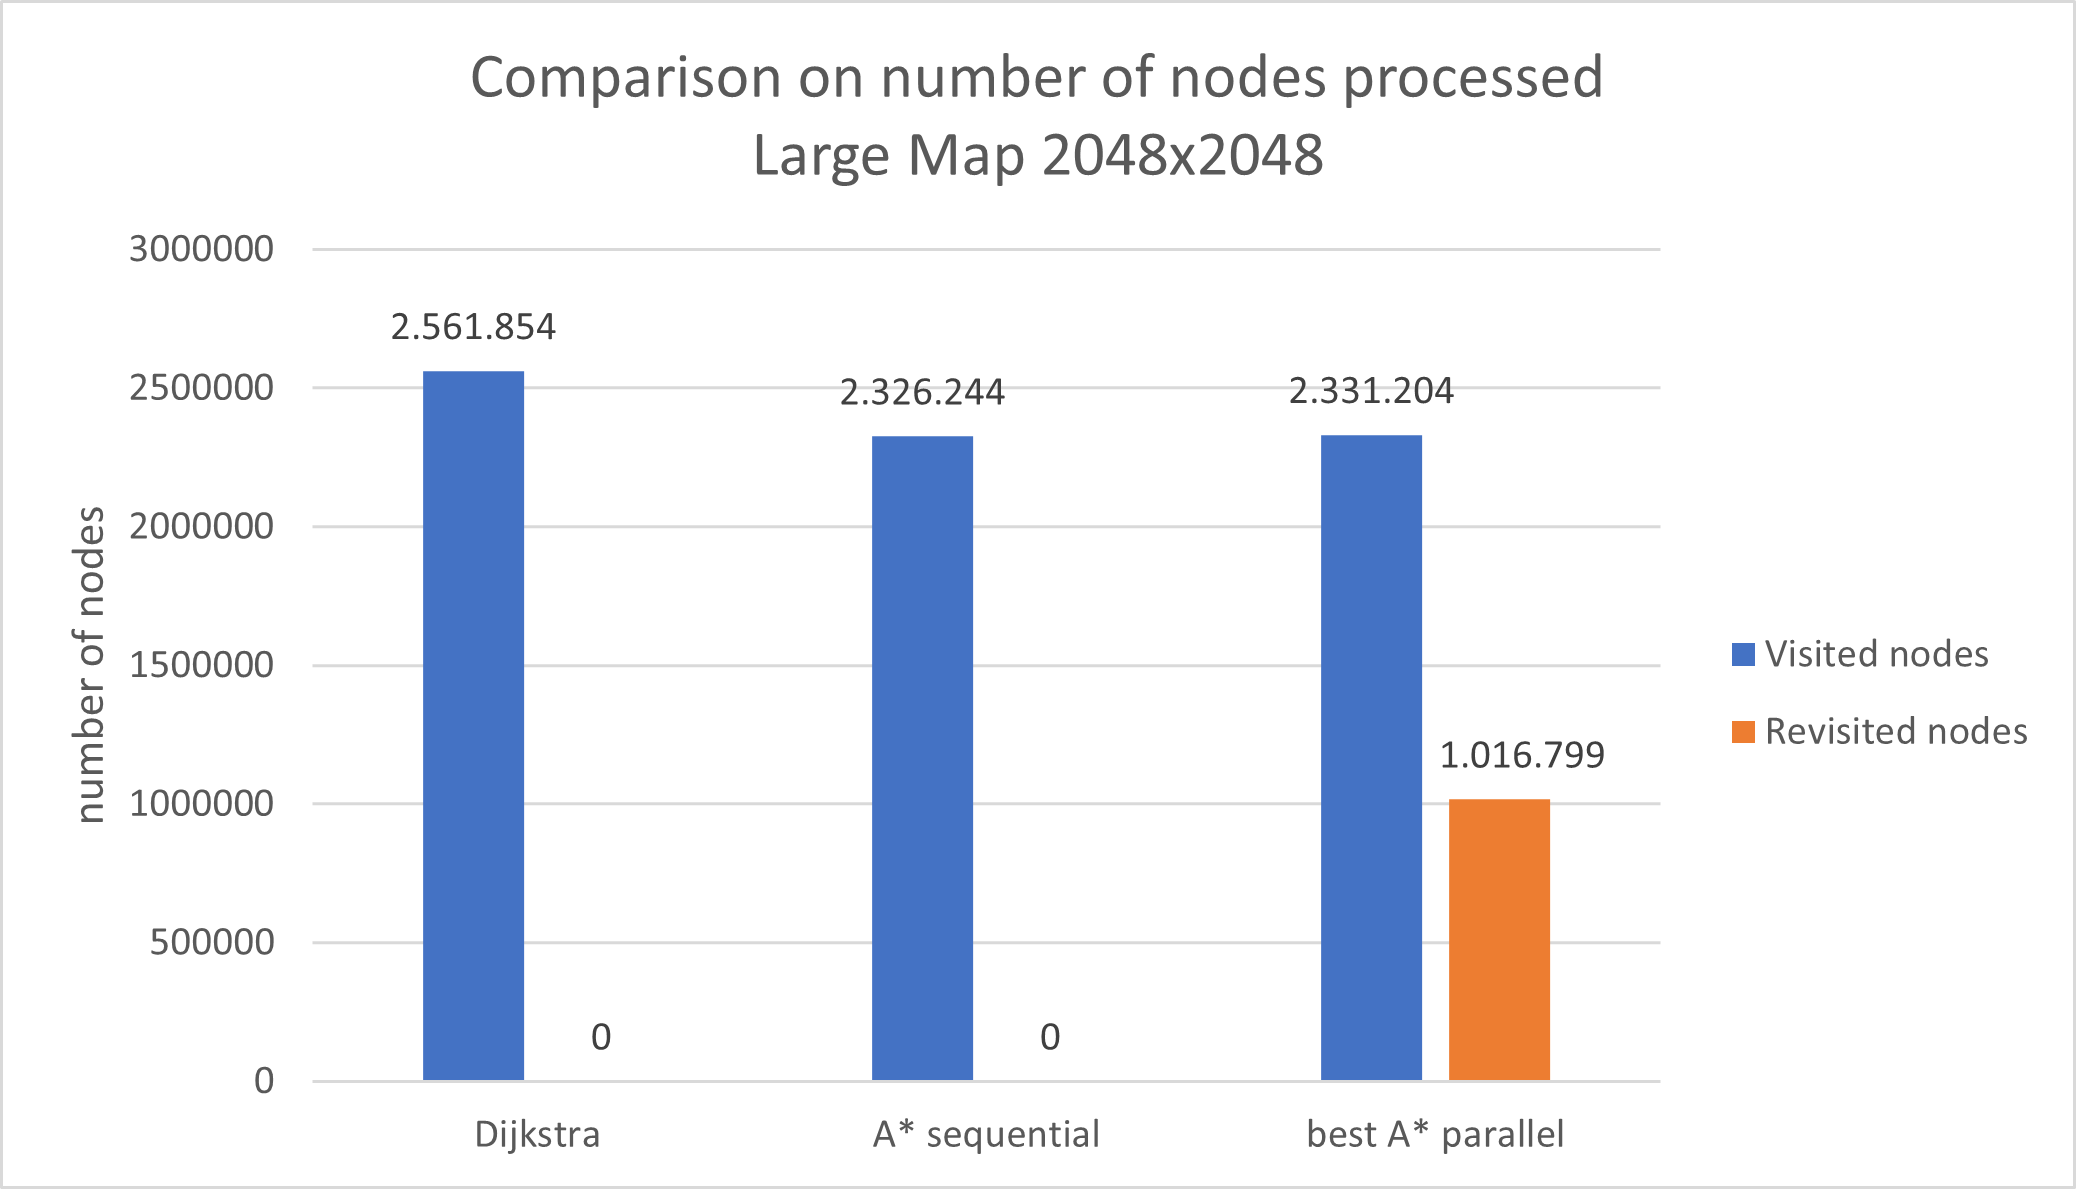
\includegraphics[scale=0.45]{mapComparisonNodes.png}
        \captionof{figure}{Performance comparison between different algorithms on large map}
        \label{Map-comp-nodes}
    \end{minipage} 
\end{center}
As we can see above (Figure \ref{Map-comp} and Figure \ref{Map-comp-nodes}), the parallel version outperforms both the sequential one and Dijkstra algorithm.
\\
Instead, the sequential version is the one which visits the least number of nodes (as expected).
\\
Since the heuristic is admissible, the sequential version does not revisit any node, while the parallel one revisits a large number of nodes due to the OPEN and CLOSED list being local to the thread.
\\
In the following page we can see a visual representation of the path found inside the map (Figure \ref{large-map}).
\newpage
\begin{figure}
    \centering
    \includegraphics{map5.png}
    \caption{Large map with path found, highlighted in red}
    \label{large-map}
\end{figure}
\noindent Now we will turn our attention to the choice of the compute recipient function.
\begin{center} 
    \begin{minipage}[b]{0.5\textwidth}
            \centering
            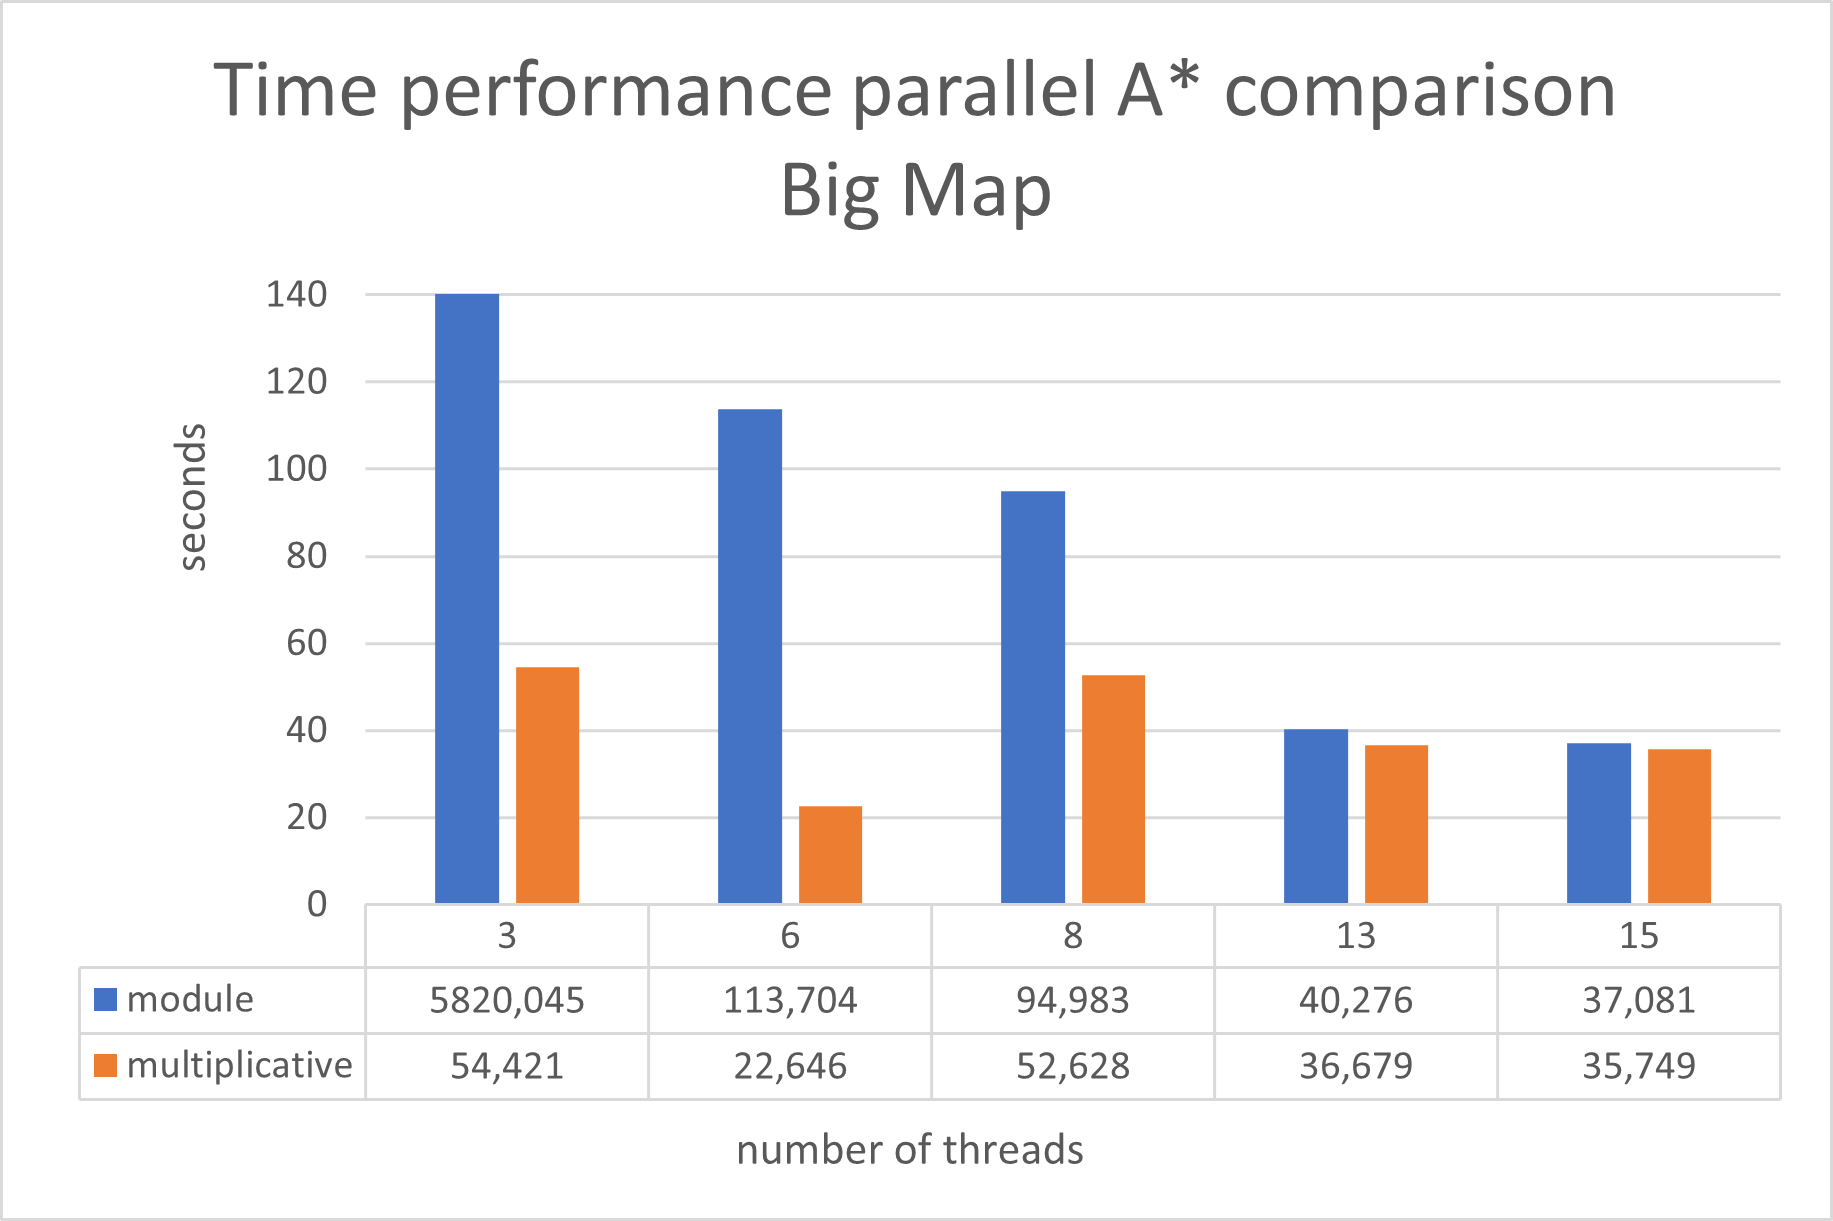
\includegraphics[scale=0.5]{mapParComparison.png}
            \captionof{figure}{Performance comparison with different number of threads and compute recipient function}
            \label{Map-par-comp}
        
    \end{minipage}%
    \hspace{1cm}
    \begin{minipage}[b]{0.4\textwidth}
            \centering
            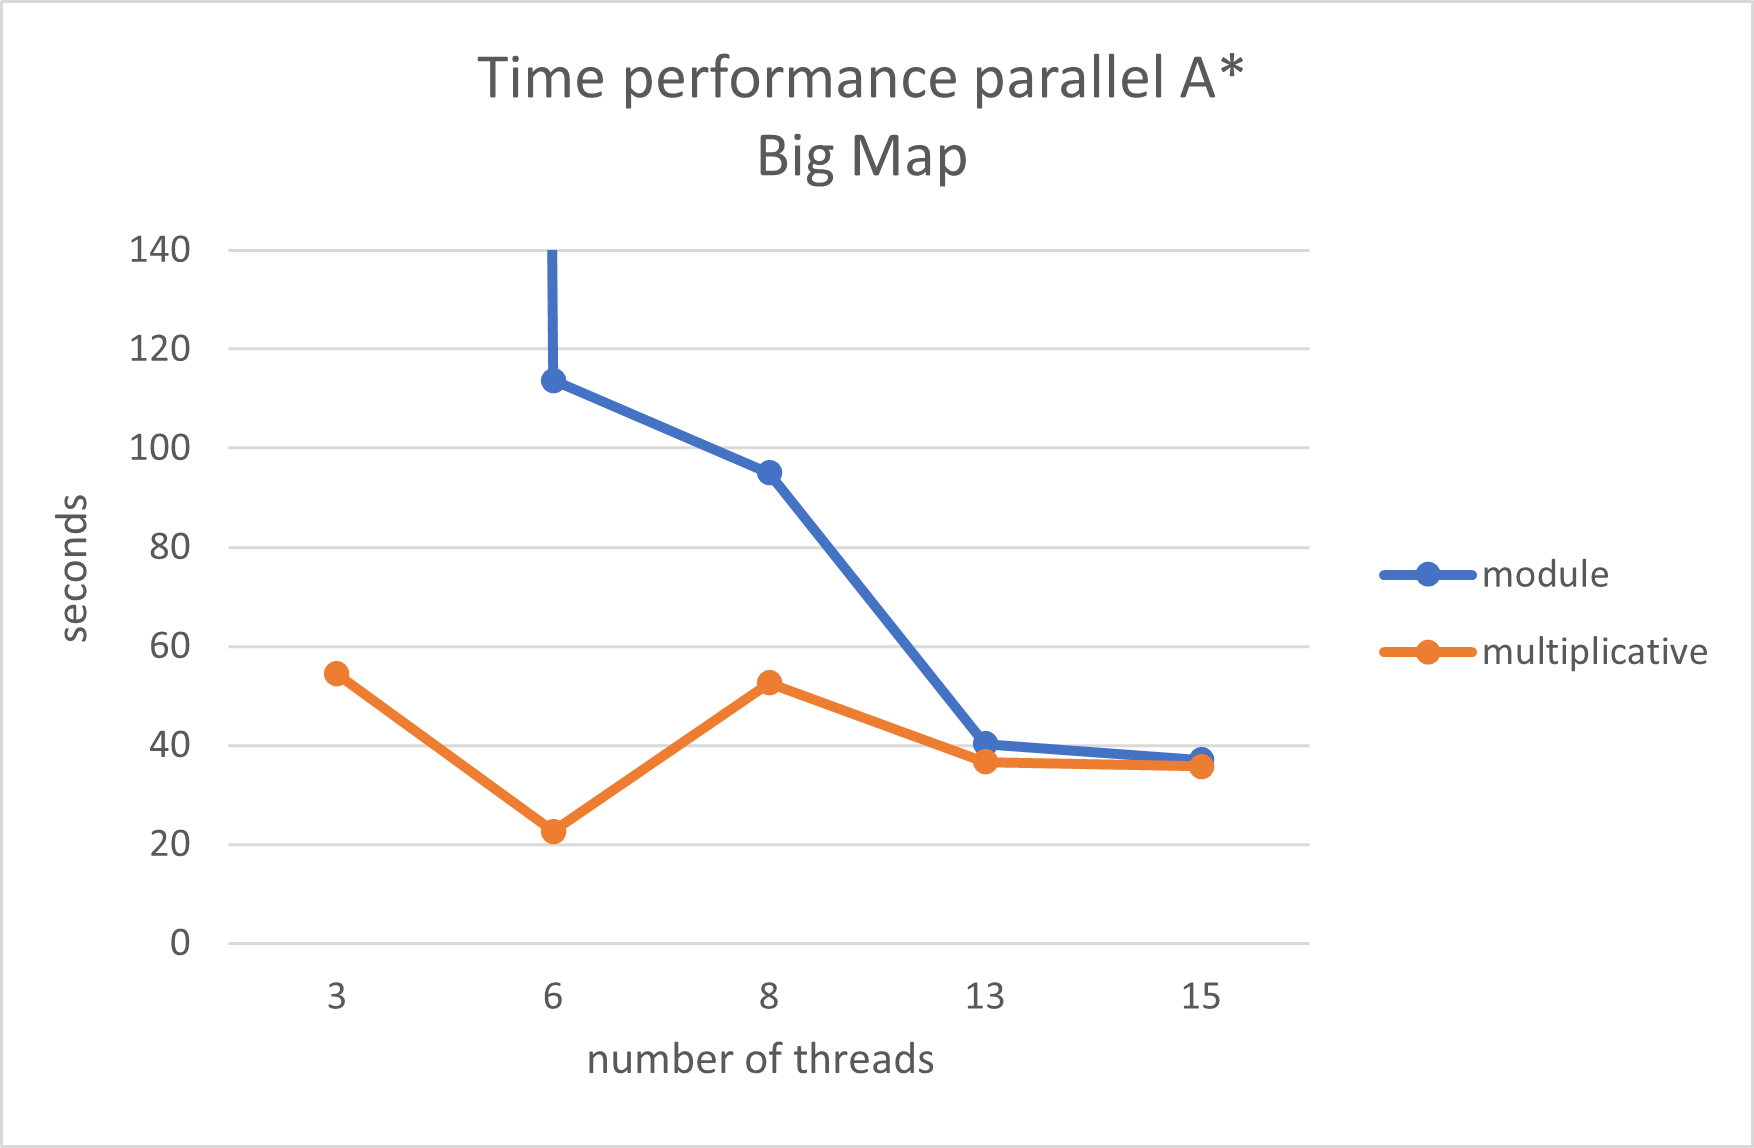
\includegraphics[scale=0.4]{mapParComparisonLines.png}
            \captionof{figure}{Tendency comparison with different number of threads and compute recipient function}
            \label{Map-par-comp-lines}
    \end{minipage} 
\end{center}
By looking at the results on Figure \ref{Map-par-comp}, it can be observed that the multiplicative hash function is more stable when changing the number of threads.
\\
For small level of parallelism (eg. 3 threads) the module hash needs almost two hours to find the correct path, while exploring and revisiting a large number of nodes.
\\
The seconds needed to find a path decrease considerably when increasing the number of threads, but for some values (mostly even values of threads eg. 12), the time to converge to a result greatly increases again.
\\
Instead, the multiplicative hash has generally better performances, but we found some limits on the number of threads (again even values from 16 onwards) beyond which the time increases.
\\
We think the problem is due to the module operation with respect to the number of threads. A possible solution is discussed later (\ref{balance_mul_hash}).

\subsection{Memory occupation}

To track the memory occupation, we used the Valgrind-Massif \cite{bibValgrind} tool, which is a heap profiler. It measures how much heap the program uses: this includes both the useful space
and the extra bytes allocated for book-keeping and alignment purposes.
\\
The graph generated by the program shows the memory occupation on specific time snapshots. The X axis indicates the bytes allocated/deallocated on the heap and stack(s), while the Y axis shows the actual memory occupation on that specific snapshot.

\vspace{0.5cm}

\begin{center}
    \begin{minipage}[b]{0.45\textwidth}
        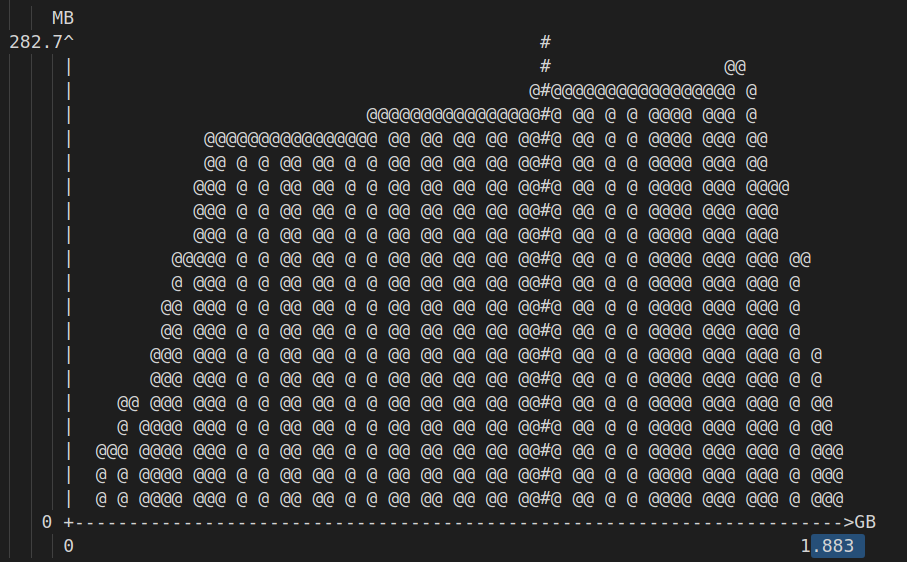
\includegraphics[scale=0.2]{mem_milan_seq.png}
        \captionof{figure}{Memory occupation of sequential A* with Milan grid}
        \label{mem-seq-milan}
    \end{minipage}
    \hspace{0.5cm}
    \begin{minipage}[b]{0.45\textwidth}
        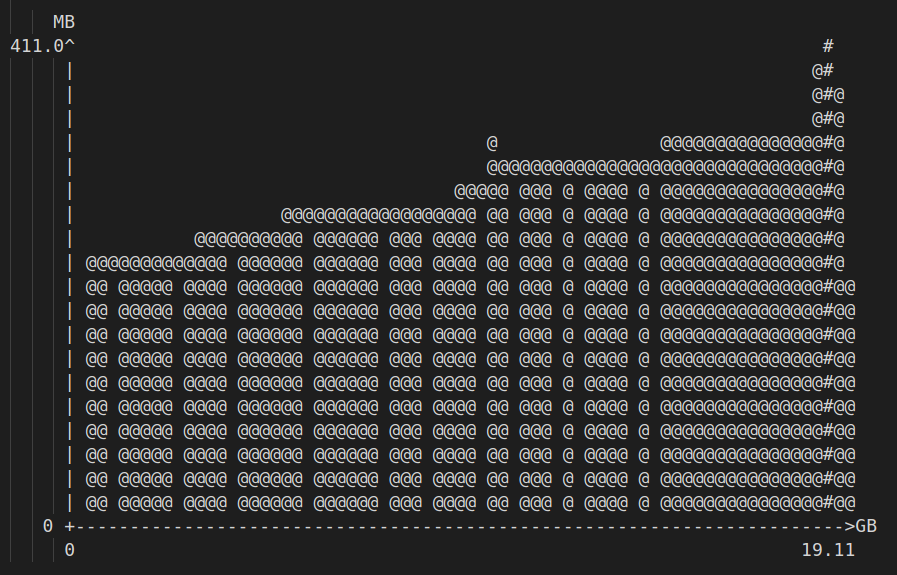
\includegraphics[scale=0.2]{mem_milan_par.png}
        \captionof{figure}{Memory occupation of parallel A* with Milan grid}
        \label{mem-par-milan}
    \end{minipage}%
    
    \vspace{0.5cm}
    
    \begin{minipage}[b]{0.45\textwidth}
        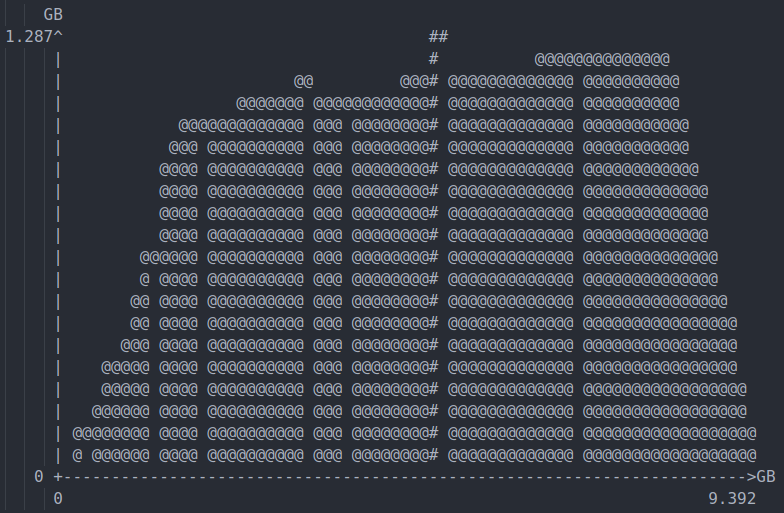
\includegraphics[scale=0.23]{mem_map_seq.png}
        \captionof{figure}{Memory occupation of sequential A* with large map}
        \label{mem-seq-map}
    \end{minipage}%
    \hspace{0.5cm}
    \begin{minipage}[b]{0.45\textwidth}
        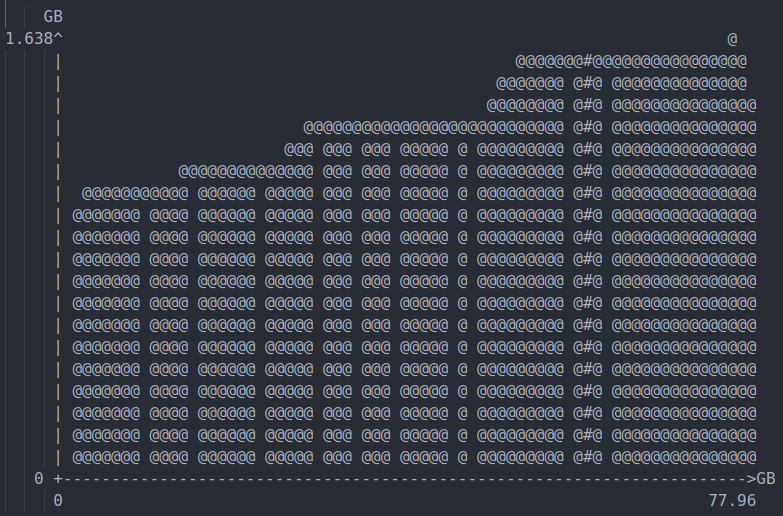
\includegraphics[scale=0.23]{mem_map_par.png}
        \captionof{figure}{Memory occupation of parallel A* with large map}
        \label{mem-par-map}
    \end{minipage}

\end{center}
It is worth to mention that more than half of the used space is occupied by the graph structure and it is not due to the algorithms.
\\
As expected, the memory occupation of the sequential A* is lower since it has only one OPEN set and one CLOSED set and it does not need to allocate additional structures for threads communication and synchronization.
It can be also noticed the difference between the sum of all the allocation made by the two algorithms (78 GB allocated totally by parallel A* on Figure \ref{mem-par-map} against 9 GB by sequential A* for the large map on Figure \ref{mem-seq-map}).
\\
To ensure that there are no memory leaks we used an option of the Valgrind tool which keeps track of all heap blocks allocated by the program.
\\
As shown in the Figure \ref{mem-leak-milan}, the algorithm does not have any memory leak.

\begin{figure}[h]
    \centering
    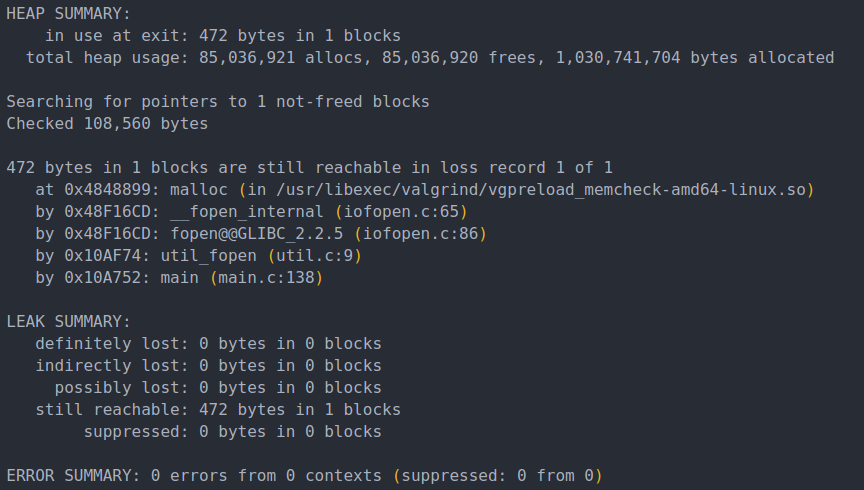
\includegraphics[scale=0.4]{mem_leak_report.png}
    \caption{Valgrind output of memory leak of parallel A* with Milan grid. The leak summary section shows the memory leaks of the program}
    \label{mem-leak-milan}
\end{figure}


